\documentclass[conference]{IEEEtran}
\IEEEoverridecommandlockouts
% The preceding line is only needed to identify funding in the first footnote. If that is unneeded, please comment it out.

%\usepackage{graphicx,times}

\usepackage[utf8x]{inputenc}
\usepackage{lmodern,textcomp}
\usepackage{multirow}
%\usepackage{subfig}
%\usepackage{caption}
\usepackage{tipa}
\usepackage{hyperref}
\usepackage{multirow}
\usepackage{verbatim}
\usepackage{booktabs}
\usepackage{booktabs,siunitx}
\usepackage{amsmath}
\usepackage[export]{adjustbox}
\usepackage{graphicx,times}
\usepackage{color}
\usepackage{mathtools}
\usepackage[english]{babel}
\usepackage[utf8x]{inputenc}
\usepackage{listings}
\usepackage{bm}

\usepackage{geometry}
 \geometry{
 a4paper,
 left=54pt,
 top=122pt,
 right=37pt,
 bottom=54pt
 }

\usepackage{cite}
\usepackage{amsmath,amssymb,amsfonts}
\usepackage{algorithmic}
\usepackage{graphicx}
\usepackage{textcomp}
\usepackage{xcolor}
\def\BibTeX{{\rm B\kern-.05em{\sc i\kern-.025em b}\kern-.08em
    T\kern-.1667em\lower.7ex\hbox{E}\kern-.125emX}}
\begin{document}


\title{Stochastic modelled grid outage effect on home Energy Management}


\author{\IEEEauthorblockN{Jesse-James PRINCE AGBODJAN}
\IEEEauthorblockA{\textit{IETR (Institut d’\'Electronique et} \\
\textit{de T\'elecommunications de Rennes)}\\
CentraleSupelec, Rennes, France \\
jesse-james.prince-agbodjan@centralesupelec.fr}
\and
\IEEEauthorblockN{Pierre HAESSIG}
\IEEEauthorblockA{\textit{IETR (Institut d’\'Electronique et} \\
\textit{de T\'elecommunications de Rennes)}\\
CentraleSupelec, Rennes, France \\
pierre.haessig@centralesupelec.fr}
\and
\IEEEauthorblockN{Romain.Bourdais}
\IEEEauthorblockA{\textit{IETR (Institut d’\'Electronique et} \\
\textit{de T\'elecommunications de Rennes)}\\
CentraleSupelec, Rennes, France \\
romain.bourdais@centralesupelec.fr}
\and
\IEEEauthorblockN{\hspace{7.2cm}Herve GHEGUEN}
\IEEEauthorblockA{\hspace{7.3cm}\textit{IETR (Institut d’\'Electronique et} \\
\hspace{7.3cm}\textit{de T\'elecommunications de Rennes)}\\
\hspace{7.3cm}CentraleSupelec, Rennes, France \\
\hspace{7.3cm}herve.gueguen@centralesupelec.fr}}


\maketitle

\begin{abstract}
This paper focuses on improving the notion of resilience of existing controllers based on Model Predictive control. The controller resulting that we have called \textit{resilient open loop feedback controller} takes into consideration a stochastic model of a default. Throughout simple transformations it is shown that the resulting problem solved by the new controller is completely deterministic although the initial problem is stochastic. An important reduction of the number of variables needed to solve the problem compare to the state of the art is also observed. Two stochastic grid outages model are considered in order to test the performances of the controller.
\end{abstract}

\begin{IEEEkeywords}
Home Energy Management System (HEMS) , Resilience, Model Predictive Control (MPC), multi objectives optimization, Open Loop Feedback Controller(OLFC)].
\end{IEEEkeywords}

\section{Introduction}
Home Energy Management System (HEMS) are based on controllers that optimize some economic criteria. This optimization is mainly done through balancing the grid, the renewable energy sources and the local storage, but the latter can also be utilize to enhance the energy independence and the resilience of the system when the grid fails. The importance of a grid failing might not be obvious but related works \cite{OnlnCER} showed that grid power outages habitually occur in off grid locations, less frequently in developed countries but when they do happen, they greatly impact people's live.

There is a lot of works on HEMS in general but a few deals with the behavior of the controller before and during an outage. Among them, \cite{HGhRBo2015,RRoFBe2014} propose reducing the user's comfort by shutting down a part of the demand as soon as the outage happens. That same idea is used in \cite{JMaHJa2016}, but an additional condition is to reserve at all time, a fixed quantity of energy storage to be used only in case of outage. In our previous work \cite{JPrPHa2019} the resilient model predictive controller uses the power of Model Predictive Control framework to dynamically choose the right level of energy within the storage when the failure happens and the part of the demand to shut down in order to increase the system resiliency.

The common thread between all the previous cited works is that they consider a deterministic model of the Grid Power Outage (GPO) i.e. one either clearly knows when the failure might happen (scheduled GPO) or not (unscheduled GPO). 
This work which follows what we have proposed in \cite{JPrPHa2019}, is different in his character by considering a stochastic model of the grid behavior. Two optimization fields  provide a framework which help resolving the resulting problem. These are Robust Optimization (RO) \cite{BenTal2009} and Probabilistic Programming (PP) \cite{Ankopa1995}. PP problem can be formulated using two different approaches, $multistage\,\, stochastic \,\, optimization$ (MSO) \cite{Ankopa1995} and  $probabilistic/chance$  $constraint (CC)$ \cite{AChWCo1958,AChWCo1959}. In this paper we are going to focus our attention on the MSO, leaving the RO and the CC in the  perspective  of  future  works.

The paper is further organized as follows. Section \ref{CaseStudy} describes briefly the main components of the system considered, recalls the control objective, states the problem at hands, presents how it can be solved using the MSO and proposes a new solution which leads to the design of the new controller in section \ref{ROLFC}. Following in section \ref{ModelGriBeh} two models of grid behavior are introduced to test its behavior.  The next section presents the results and some analysis of the different simulations. Conclusion and future directions are given at the end in section~\ref{conclusion}.


\section{Case Study}\label{CaseStudy}

\quad The Case Study is a solar home represented by its power flow model (Fig.~\ref{fig:solhome}). It is a discrete time model of a photovoltaic system with storage for the self-consumption of a residential consumer connected to the electrical grid. It is comprised of 2 external known variables $P_{pv}^{max}$, $P_l^*$ respectively the solar potential production  and the power demand of the house (in red) and 4 controlled variables $P_g$, $P_{sp}$, $P_b$ and $P_s$ (in green) defined as follow : \newgeometry{left=54pt,top=104pt,right=37pt,bottom=54pt}
\begin{itemize}
\item $P_g$ is the power drawn from the grid bounded bellow and above
respectively by 0 (selling energy is not authorized) and the maximum power subscribed by the user $P_g^{max}$,
\item $P_{sp}$ is the spilled solar power when it cannot be used directly or stored, therefore $P_{pv}$ the actual solar 
energy used in the system is the difference between $P_{pv}^{max}$ and $P_{sp}$, $P_{pv} = P_{pv}^{max}-P_{sp}$
\item $P_s$ the shedded power representing the energy not provided to the load (house), hence the actual power provided to the load $P_l = P_l^* - P_s$
\item $P_b$ the power into/out of the storage unit, which accumulation over time gives the energy in the battery $E_b$, constrained above by $E_b^{max}$ the maximum capacity of the battery. 
\end{itemize}
\subsection{Solar home control objective }

For the solar home, the base controller has two objectives:
\begin{itemize}
    \item ObjA: Minimizing the electricity bill given by $\sum C_gP_g$, where $C_g$ is the electricity price
    \item ObjB: Minimizing the  discomfort bill given by $\sum C_sP_s$, where $C_s$ is a virtual price associated with a unit of discomfort
\end{itemize}
The multi-objectives problem A and B is converted into a single objective optimization problem through linear scalarization \cite{Deb2014} where the objectives A and B are aggregated with positive weights which serve to normalize the main cost functions as well as organize the sub-objectives function
priority. Since the price of the electricity (the weight associated with ObjA) is a problem input, our only degree of freedom is the weight associated with ObjB ($C_s)$ that we choose to be higher than that of ObjA, i.e. $C_s \gg max(C_g)$ to transcribe the fact that avoiding the discomfort is more important than paying a lower electricity bill. Note that the electricity price can vary during the day.

The problem to be solved is therefore completely  described by:
\begin{subequations}
    \begin{align} 
        & \underset{P_g,P_{sp},P_b,P_s}{\text{min}} J = \sum_{k=1}^{N} C_gP_g + C_sP_s \label{eq:cost2min}\\
        & \text{\hspace{20px} s.t.\hspace{15px}} 0 \leq P_g \label{eq:Pgr_cons1} \\
        & \hspace{52px} P_g\leq P_g^{max} \label{eq:Pgr_cons2}\\
        & \hspace{52px} 0 \leq P_{sp} \leq P_{pv}^{max} \label{eq:Pcu_cons}\\
        & \hspace{52px} 0 \leq P_s \leq P_l^* \label{eq:Psh_cons} \\
        & \hspace{52px} 0 \leq E_b \leq E_b^{max} \label{eq:Est_cons} \\
        & \hspace{52px} P_{pv}^{max}-P_{sp} = P_{pv} \label{eq:P_pv} \\
        & \hspace{52px} P_l^* - P_s =  P_l\label{eq:P_l} \\
        & \hspace{52px} E_b(k+1) = E_b(k) + P_b(k)\Delta_t \label{eq:Est_dyn}  \\
        & \hspace{52px} P_g- P_b + {P_{pv}} = P_l \label{eq:Engy_csvt} 
    \end{align}
\end{subequations}

\begin{figure}[!t]

    \begin{center}
                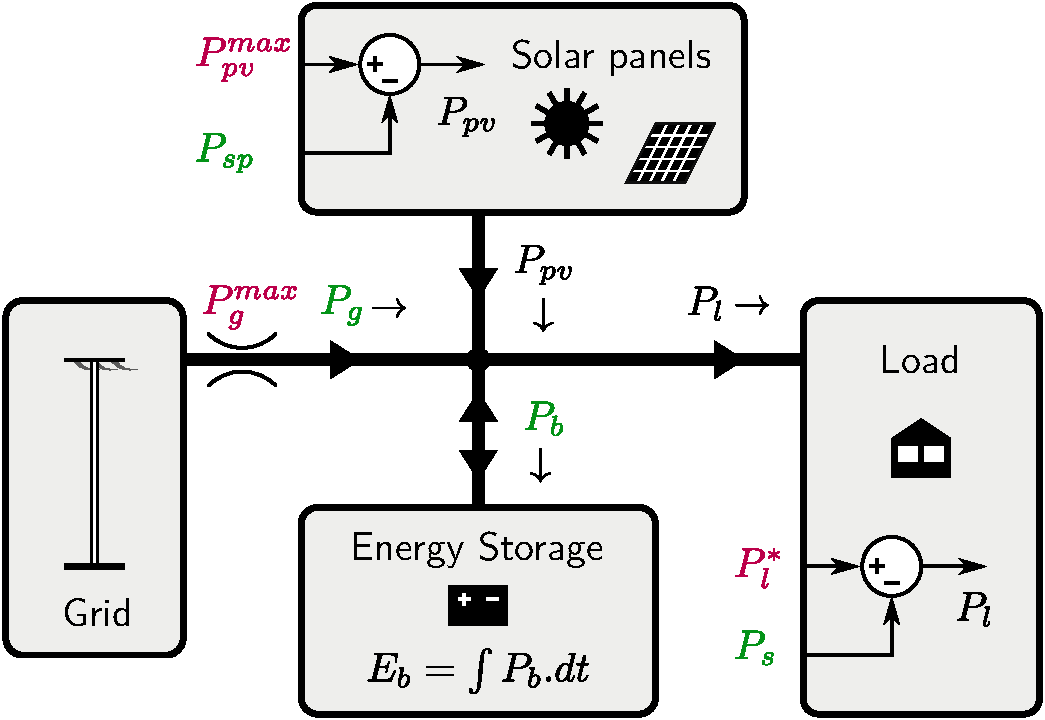
\includegraphics[width=0.8\columnwidth]{Figures/solar_home_compact.pdf}
        \end{center}

        \caption{Power flow model of a solar home.
        The decision/controlled variables are colored in green, external data are colored in red (Solar potential and desired consumption), internal variables are colored in black.
        }
        \label{fig:solhome}
   
\end{figure}

Note that all the variables and constraints of the previous problem are evaluated at each instant $k \in \{1, \ldots, N \}$, i.e. should therefore been indexed by `` $k$ '' but we have deliberately choose not to  put it for clarity and simplicity sake as we will do for the rest of the paper.

Introduced in the model Predictive Control (MPC) framework \cite{ECaCbo2007}, the previous problem is now solved over a sliding horizon H and becomes : 
\begin{equation}\label{eq:MPCsys}
\left. 
\begin{aligned}
&U_k = \text{argmin } J_H = \sum_{j=k}^{k+H} C_gP_g + C_sP_s, \hspace{3px} \forall k \in [1, N] \\
& \text{\hspace{50px} s.t.\hspace{15px}} (\ref{eq:Pgr_cons1}),(\ref{eq:Pgr_cons2}),(\ref{eq:Pcu_cons}),(\ref{eq:Psh_cons}), (\ref{eq:Est_cons}),  (\ref{eq:P_pv}),\\
& \text{\hspace{157px}}(\ref{eq:P_l}), (\ref{eq:Est_dyn}),(\ref{eq:Engy_csvt})
\end{aligned}\right \}
\end{equation}

\begin{figure}[!b]
         \centering
    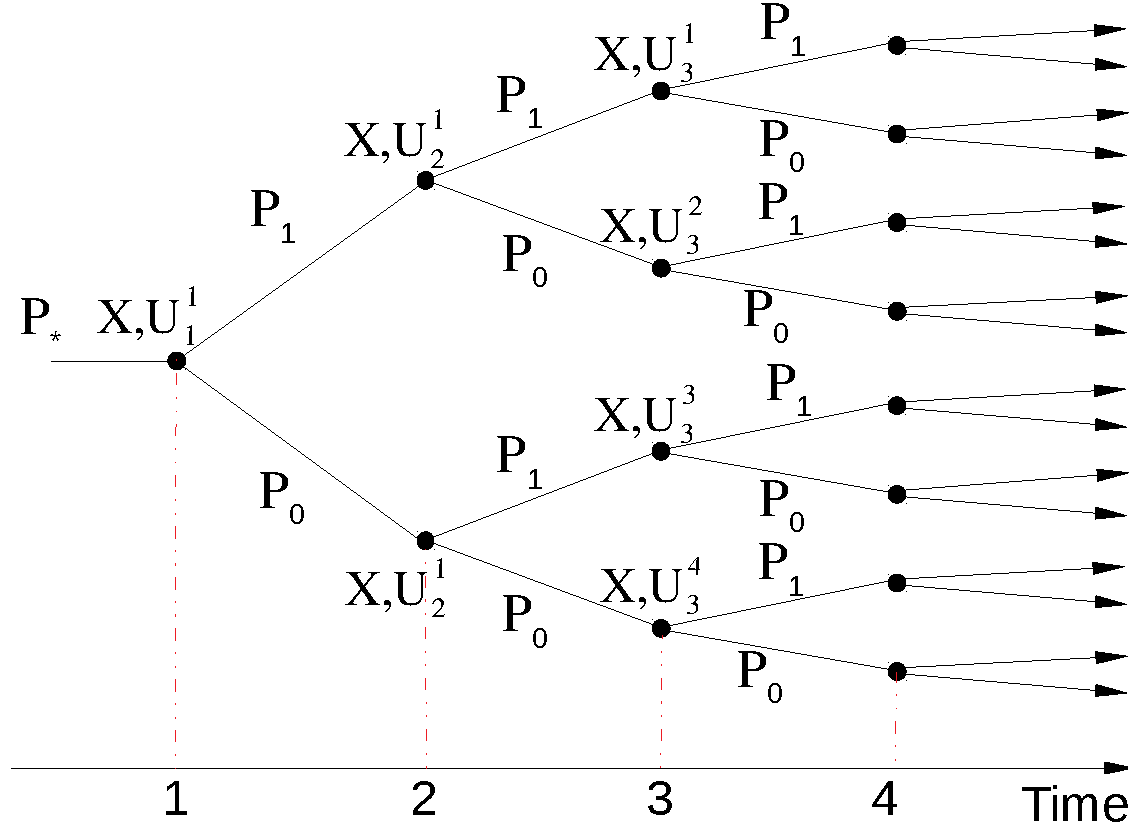
\includegraphics[width=0.80\columnwidth]{Figures/treePaper2.pdf}
    \caption{Scenario tree representation of the uncertainty evolution for multi-stage optimisation with $X_*^*$, $U_*^*$ and $P_*$ respectively the dynamic state of the system, the control and the uncertainty. Note that at  the initial time 1  the uncertainty has already revealed. 
}
    \label{fig:Snr_tree}
\end{figure}
\noindent where $U_k = [u(k), u(k+1), \ldots,u(k+H-1), u(k+H)]$, with  $u = [ P_g,P_{sp},P_b,P_s]'$ and only the first control $u(k)$ is applied to the system at instant k. The same process is repeated at each instant. 
\subsection{Problem statement}
If the trajectory of all the problem's inputs i.e. $P_l^*$, $P_{pv}^{max}  \text{ and } P_g^{max}$ are known in advance, solving it is straight because we obtain a deterministic optimization problem. 
That is the case that has been treated in \cite{JPrPHa2019}. In the other hand let us consider now the case where $\textbf{P}_\textbf{g}^{\textbf{max}}$ \footnote{From now on we are going to differentiate  a r.v. by writing it in bold}  is a random variable (r.v.) taking its value in a set $\mathcal{P}$ defined as $ \mathcal{P} = \left \{ P_0 , P_1\right \}$. Note that $P_0=0$ and $P_1$ is the maximum power subscribed by the user. More Explicitly if the r.v. : \begin{itemize}
\item $P_g^{max} = P_0 \rightarrow$ the grid is not available, an outage is occurring ; 
\item $P_g^{max} = P_1 \rightarrow$ the grid is available and we can draw energy from it . 
\end{itemize}

Taking into consideration the stochastic characteristic of $\textbf{P}_\textbf{g}^{\textbf{max}}$, problem (\ref{eq:MPCsys}) is ill defined since we do not know how to evaluate  neither constraint (\ref{eq:Pgr_cons1}) nor the cost (\ref{eq:cost2min}).
 
 The structure of the problem (2) is such that some variables can act as recourse. Therefore its natural and direct extension to PP is the MSO. The latter consider all the possible realizations of a r.v. and resolve an unique optimization problem. The size of the resulting problem grows exponentially in consonance with the distribution of the r.v. and the number of instant considered. Let L be the number of control and state variable of the optimization problem at one instant, $|\Omega|$ be the size of the r.v. sample space and M the number of instant considered in the future. The MSO problem associated yields exactly  $L|\Omega|^M$ variables. Fig. \ref{fig:Snr_tree} shows   the scenario tree for $|\Omega|= 2$ and M=5. 
  
To deal with the exponential growth of the scenario tree in MSO, the authors in \cite{SLuAJo2014} assume that the uncertainty becomes a constant after some point in time.  In this paper we do not go in that direction since the nature of the uncertainty considered here is the type on/off. Due to the structure of our problem, the controller we have come up with is based on the $Open\, loop\, feedback$ framework as in \cite{YBarRSi1969} 
 
 \section{The resilient open loop feedback controller (OLFC)}\label{ROLFC}
\begin{table*}[!htbp]
%% increase table row spacing, adjust to taste
\renewcommand{\arraystretch}{1}
\caption{Controller Performances for both Low and High failure rate}
\noindent
\centering
  \begin{minipage}{\linewidth} %Use the minipage environment to footnote tables
 
        \begin{center}
            \begin{tabular}{c||*{4}{c|}c||*{4}{c|}c||}
		\cline{2-11}
	
	 &\multicolumn{5}{c||}{\textbf{No outage}} & \multicolumn{5}{c}{\textbf{With outage}} \\ \cline{2-11}
	
	
	  &\multirow{2}{*}{$\sum P_{g}dt$} & \multirow{2}{*}{$\sum P_{s}dt$}
	& \multicolumn{3}{c||}{\begin{tabular}[c]{@{}c@{}}$E_b$\end{tabular}} &\multirow{2}{*}{$\sum P_{g}dt$}  &\multirow{2}{*}{$\sum P_{s}dt$} &\multicolumn{3}{c||}{\begin{tabular}[c]{@{}c@{}}$E_b$\end{tabular}}\\ \cline{1-1}\cline{4-6}  \cline{9-11} 
	
	 $\lambda$ &  &  &Beg &Mid  &End &   &   &Beg   &Mid   &End \\\cmidrule[1pt]{1-11}
	 Low  &19.3   &\multirow{2}{*}{0}    &\multirow{2}{*}{0}  &0.2   &0   &4.7  &14.6  &\multirow{2}{*}{0}    &0.2    &\multirow{2}{*}{0} \\ \cline{1-1}
	 High &26.7   &   &  &4.5 &7.4 &9.0  &10.3  &  &4.5  & \\\cmidrule[1pt]{1-11}
	        \end{tabular}
        \end{center} \label{tab:CompTable1}
    \end{minipage}
\end{table*} 
Consider problem (\ref{eq:MPCsys}) which is the minimization of the cost $J_H$ over the horizon $[k, \, k+H$]. Assuming that the r.v. has revealed already for the initial time $k$ but not for the future $[k+1, \, k+H$], the problem to be solved is that  we need to choose how much energy must be drawn from the grid before we know if the latter is available or not. 

Provided that the lower bond on the r.v. $\bm{P_g^{max}}$ equals the left hand side of (\ref{eq:Pgr_cons1}), the latter  is always satisfied. 

Consider now the constraint (\ref{eq:Pgr_cons2}) namely $P_g(j)\leq \bm{P_g^{max}}$, $\forall j \in [k+1,\, k+H]$. Since we do not know in advance the value that the r.v. will take,  let us suppose that at a certain instant $ j \in [k+1, \, k+H$], $P_0 < P_g(j) < P_1$. If $P_g^{max} = P_1$, the constraint (\ref{eq:Pgr_cons2}) is satisfied. On the contrary if $P_g^{max} = P_0$, the constraint (\ref{eq:Pgr_cons2}) is violated and the problem has no solutions. To avoid this situation we relaxed (\ref{eq:Pgr_cons2}) by introducing in a virtual external power source ($P_{ex}$) that will substitute $P_g^{max}$ when the latter takes on the value $P_0$ as follow: 
\begin{align}
     P_{g} & \leq \bm{P_g^{max}} + P_{ex}, \label{NewCons1}\\
     P_{ex} & \geq \label{NewCons2}0.
\end{align}
The usage of $P_{ex}$ is minimized, hence we add $C_{ex}P_{ex}$ ($C_{ex}$ is the cost of using the external virtual source) to the previous optimization cost such that: 
\begin{equation}
    J_{OLFC} = J_H + \sum_{j=k+1}^{k+H} P_{ex}(j)C_{ex}(j).
\end{equation}
Note that since (\ref{NewCons1}) can be rewritten as a set of the following deterministic constraints 
 \begin{align}
 P_g - P_{ex} &\leq P_1 ,\label{NewCons3}\\ 
 P_g - P_{ex} & \leq P_0,\label{NewCons4}
 \end{align}
 and that we minimize the usage of $P_{ex}$ (with an unit cost $C_{ex} \gg C_g$) we have 
 \begin{equation}
    P_{ex} = \left \{
        \begin{aligned}
            0 & \text{ if }  P_g^{max} = P_1 \\
            P_g &\text{ if } P_g^{max} = P_0.
        \end{aligned}\right.
\end{equation}
 Note that $\forall j \in [k+1, k+H] $ , $P_{ex}$ is a r.v. since it depends on the realisation of the r.v. $\bm{P_{g}^{max}}$ at those time. It follows that instead of minimizing the cost $J_{OLFC}$, we are going to minimize it's expectation
\begin{equation}
    \begin{split}
        \mathbb{E}[J_{OLFC}] &=\mathbb{E}[J_H + \sum_{j=k+1}^{k+H}C_{ex}P_{ex}] \hspace{70px} \\
                             &=\sum_{j=k}^{k+H}  C_sP_s(j) + C_g(j)P_g(j) + \\ &\hspace{20px}\pi_{1,k}(j)C_{ex}P_{ex}(j) + \pi_{0,k}(j)C_{ex}P_{ex}(j)\\
                             &=\sum_{j=k}^{k+H}  C_sP_s(j) + C_g(j)P_g(j) + \\ &\hspace{92px} \pi_{0,k}(j)C_{ex}P_{ex}(j)\\
    \end{split}
\end{equation}where $\pi_{1,k}(j)$  and $\pi_{0,k}(j)$ are respectively the probability that the default did not happen (grid is available) or has happened (grid unavailable) at instant $j$ given that the default  state is known at the initial instant $k$.

The complete problem solved by OLFC is therefore given by: 

\begin{equation}\label{eq:OLFCsys}
\left. 
\begin{aligned}
&\underset{P_g,P_{sp},P_b,P_s,P_{ex}}{\text{min}} \hspace{0px} \sum_{j=k}^{k+H}  C_sP_s(j) + C_g(j)P_g(j) +\\ & \hspace{130px} \pi_{0,k}(j)C_{ex}P_{ex}(j)\\  \\
& \text{\hspace{25px} s.t.\hspace{15px}}(\ref{eq:Pgr_cons1}),(\ref{eq:Pcu_cons}),(\ref{eq:Psh_cons}),(\ref{eq:Est_cons}),(\ref{eq:P_pv}),(\ref{eq:P_l}),\\
& \hspace{120px}(\ref{eq:Est_dyn}),(\ref{eq:Engy_csvt}),(\ref{NewCons2}),(\ref{NewCons3}),(\ref{NewCons4})
\end{aligned}\right \}
\end{equation}
The advantage of the new formulation is not only that it reduces greatly the size of the problem compare to the MSO $((L+1)M$ vs $L|\Omega|^M)$ but, more importantly is that it can be used with any type of model of faulty behavior as long as one can compute and quantify the availability $\pi_{1,k}$ or the nonavailability $\pi_{0,k}$ of the considered default throughout the time. 


\section {Model of the grid behavior}\label{ModelGriBeh}
In order to test the performances of the ROLFC, let us compute the availability $\pi_1^*$ and non availability $\pi_0^*$ of the electricity grid. Two frameworks which are the Bernoulli process  and the Markov Chain (MC)\cite{RBiRna1992} are used. 
 \subsection{Bernoulli process model of the electrical grid}
 The Bernoulli process (BP) is a (finite) sequence of identically distributed and independent (iid) r.v. that can only takes two values. The probability mass function of the r.v  $P_g^{max}$ representing the state of the  grid is then given by :
 \begin{itemize}
    \item $\mathbb{P}(P_g^{max} = P_0) = \hspace{7px}\lambda \hspace{9px} = \pi_0 $
    \item $\mathbb{P}(P_g^{max} = P_1)= 1-\lambda= \pi_1$ 
\end{itemize}
At each instant $k$, the probability of the grid being unavailable and available respectively are therefore given by $\lambda$ and $ 1-\lambda$

\subsection{Markov Chain model of the electrical grid }
 We modeled the grid secondly by a two states Markov chain given by fig. \ref{fig:MarChain} where $\lambda$ is said to be the $failure \; rate$ while $\mu$ is the $repair\; rate$.
 \begin{figure}[!ht]
        \begin{center}
                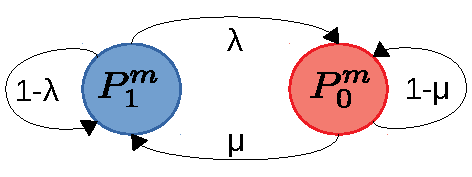
\includegraphics[width=0.60\columnwidth]{Figures/MarChain_paper.pdf}
        \end{center}
        \caption{Markov chain model of the electrical grid}
        \label{fig:MarChain}
\end{figure}
Consider that the process modelled by the different states of the electrical grid takes either the value $P_1$ when the grid is available or $P_0$ when the grid is unavailable. Let's $P^{max}_{g,k}$ denote its value at time period $k$. It follows that if $P_{g,k}^{max} = P_0$ or $P_{g,k}^{max} = P_1$ respectively the process is said to be in state unavailable and available at time $k$. Whenever the process is in some state, there is a fixed probability that it will be next in the other state or remain in the same. That is: 
\begin{subequations}\label{eq:MarChain}
\begin{align}
    \mathbb{P} \lbrace P^{max}_{g,k+1} =  P_0 | P^{max}_{g,k} = P_1, \ldots, X_0 \rbrace  &= \lambda, \\
    \mathbb{P} \lbrace P^{max}_{g,k+1} =  P_1 | P^{max}_{g,k} = P_1, \ldots, X_0 \rbrace  &= 1-\lambda, \\
    \mathbb{P} \lbrace P^{max}_{g,k+1} =  P_1 | P^{max}_{g,k} = P_0, \ldots, X_0 \rbrace  &= \mu, \\
    \mathbb{P} \lbrace P^{max}_{g,k+1} =  P_0 | P^{max}_{g,k } = P_0, \ldots, X_0 \rbrace  &= 1-\mu,
\end{align}
\end{subequations}

where, $X_0$, $P^{max}_{g,k}$ and $P^{max}_{g,k+1}$ represent respectively all the past,  present and the future states. 

Equation (\ref{eq:MarChain}) states that, for the MC represented in Fig. \ref{fig:MarChain}, the conditional distribution of any future state $P^{max}_{g,k+1}$ given all the past states resumed in $X_0$ and the present state $P^{max}_{g,k}$ is independent of the past states and
depends only on the present state. The one step transition probabilities matrix representing the MC is then given by: 
\begin{equation}\label{eq:MarChain_TransMat}
\mathbf{T} = 
  \begin{bmatrix}
 1-\lambda  & \lambda \\ 
 \mu & 1- \mu
\end{bmatrix} . 
\end{equation}

Let's denote by $\Pi^n$ the n-step transition probability vector of the process. The \textit{Chapman–Kolmogorov equations} provide a method for computing this n-step  transition probability vector such that: 
\begin{subequations}
    \begin{align}
    \Pi^n & = \Pi^0 \, \mathbf{T}^n, \quad \forall n \geq 1 \label{eq:nsStaVec1} \\
          & = \bigl[ \underbrace{\mathbb{P} (P_g^{max} = P_1 | \Pi^0)}_{\pi_{1,\cdot}(n)}\quad \underbrace{\mathbb{P} (P_g^{max} = P_0 | \Pi^0)}_{\pi_{0,\cdot}(n)} \bigl] \label{eq:nsStaVec2},
\end{align}
\end{subequations}
where the first and the second column of equation (\ref{eq:nsStaVec2}) represent respectively the probability of the grid being available ($\pi_{1,\cdot}(n))$ or unavailable $(\pi_{0,\cdot}(n))$ at time $n$ given that the initial (present) state probability vector  is $\Pi^0$. At the present state we know if the electrical grid is available or not, hence $\Pi^0$ taking either the value $[1\;0]$ when the grid is available and $[0\;1]$ on the contrary.


 \section{Simulation and results}
 
 \subsection{Simulation settings}
 All of the simulations have been done using \href{http://www.juliaopt.org/}{Julia} a high-level, high-performance dynamic programming language for technical computing with the JuMP toolbox and \href{https://www.mosek.com/}{Mosek} solver. 
 
 These simulations use a data extracted from ``\href{https://www.ausgrid.com.au/Common/About-us/Corporate-information/Data-to-share/Solar-home-electricity-data.aspx}{Solar home electricity data}'', a dataset of the Australian electricity distribution company Ausgrid. The dataset comprises of the home consumption ($P_l^*$) of several users and the solar potential ($P^{max}_{pv}$) recorded at the frequency of 30 minutes. The simulation is carried over three successive days chose randomly. We suppose that the grid failure occurs at 12:00 a.m right at the beginning the second day (denoted by a red doted vertical line on Fig. \ref{fig:LOwFailYesOut}, \ref{fig:HighFailYesOut} and remains until the end of the simulation. A whole day (H= 48 i.e. 24h) is considered as prediction horizon and $C_{g}$ consist of two energy prices defined as follow : 
\begin{itemize}
 \item $C_{night}$ : Off-peak hour, from 12:00 a.m. to 6:00 a.m (highlighted in light blue on Fig. \ref{fig:LOwFailNoOut}, \ref{fig:HighFailNoOut}, \ref{fig:LOwFailYesOut}, \ref{fig:HighFailYesOut})
 \item $C_{day}$ : peak hour from 6:30 a.m. to 23:30 p.m
\end{itemize}

 
 \subsection{Simulation results and analysis}
 
 \begin{figure*}[!ht]
  
    \begin{minipage}{.49\linewidth}
       
        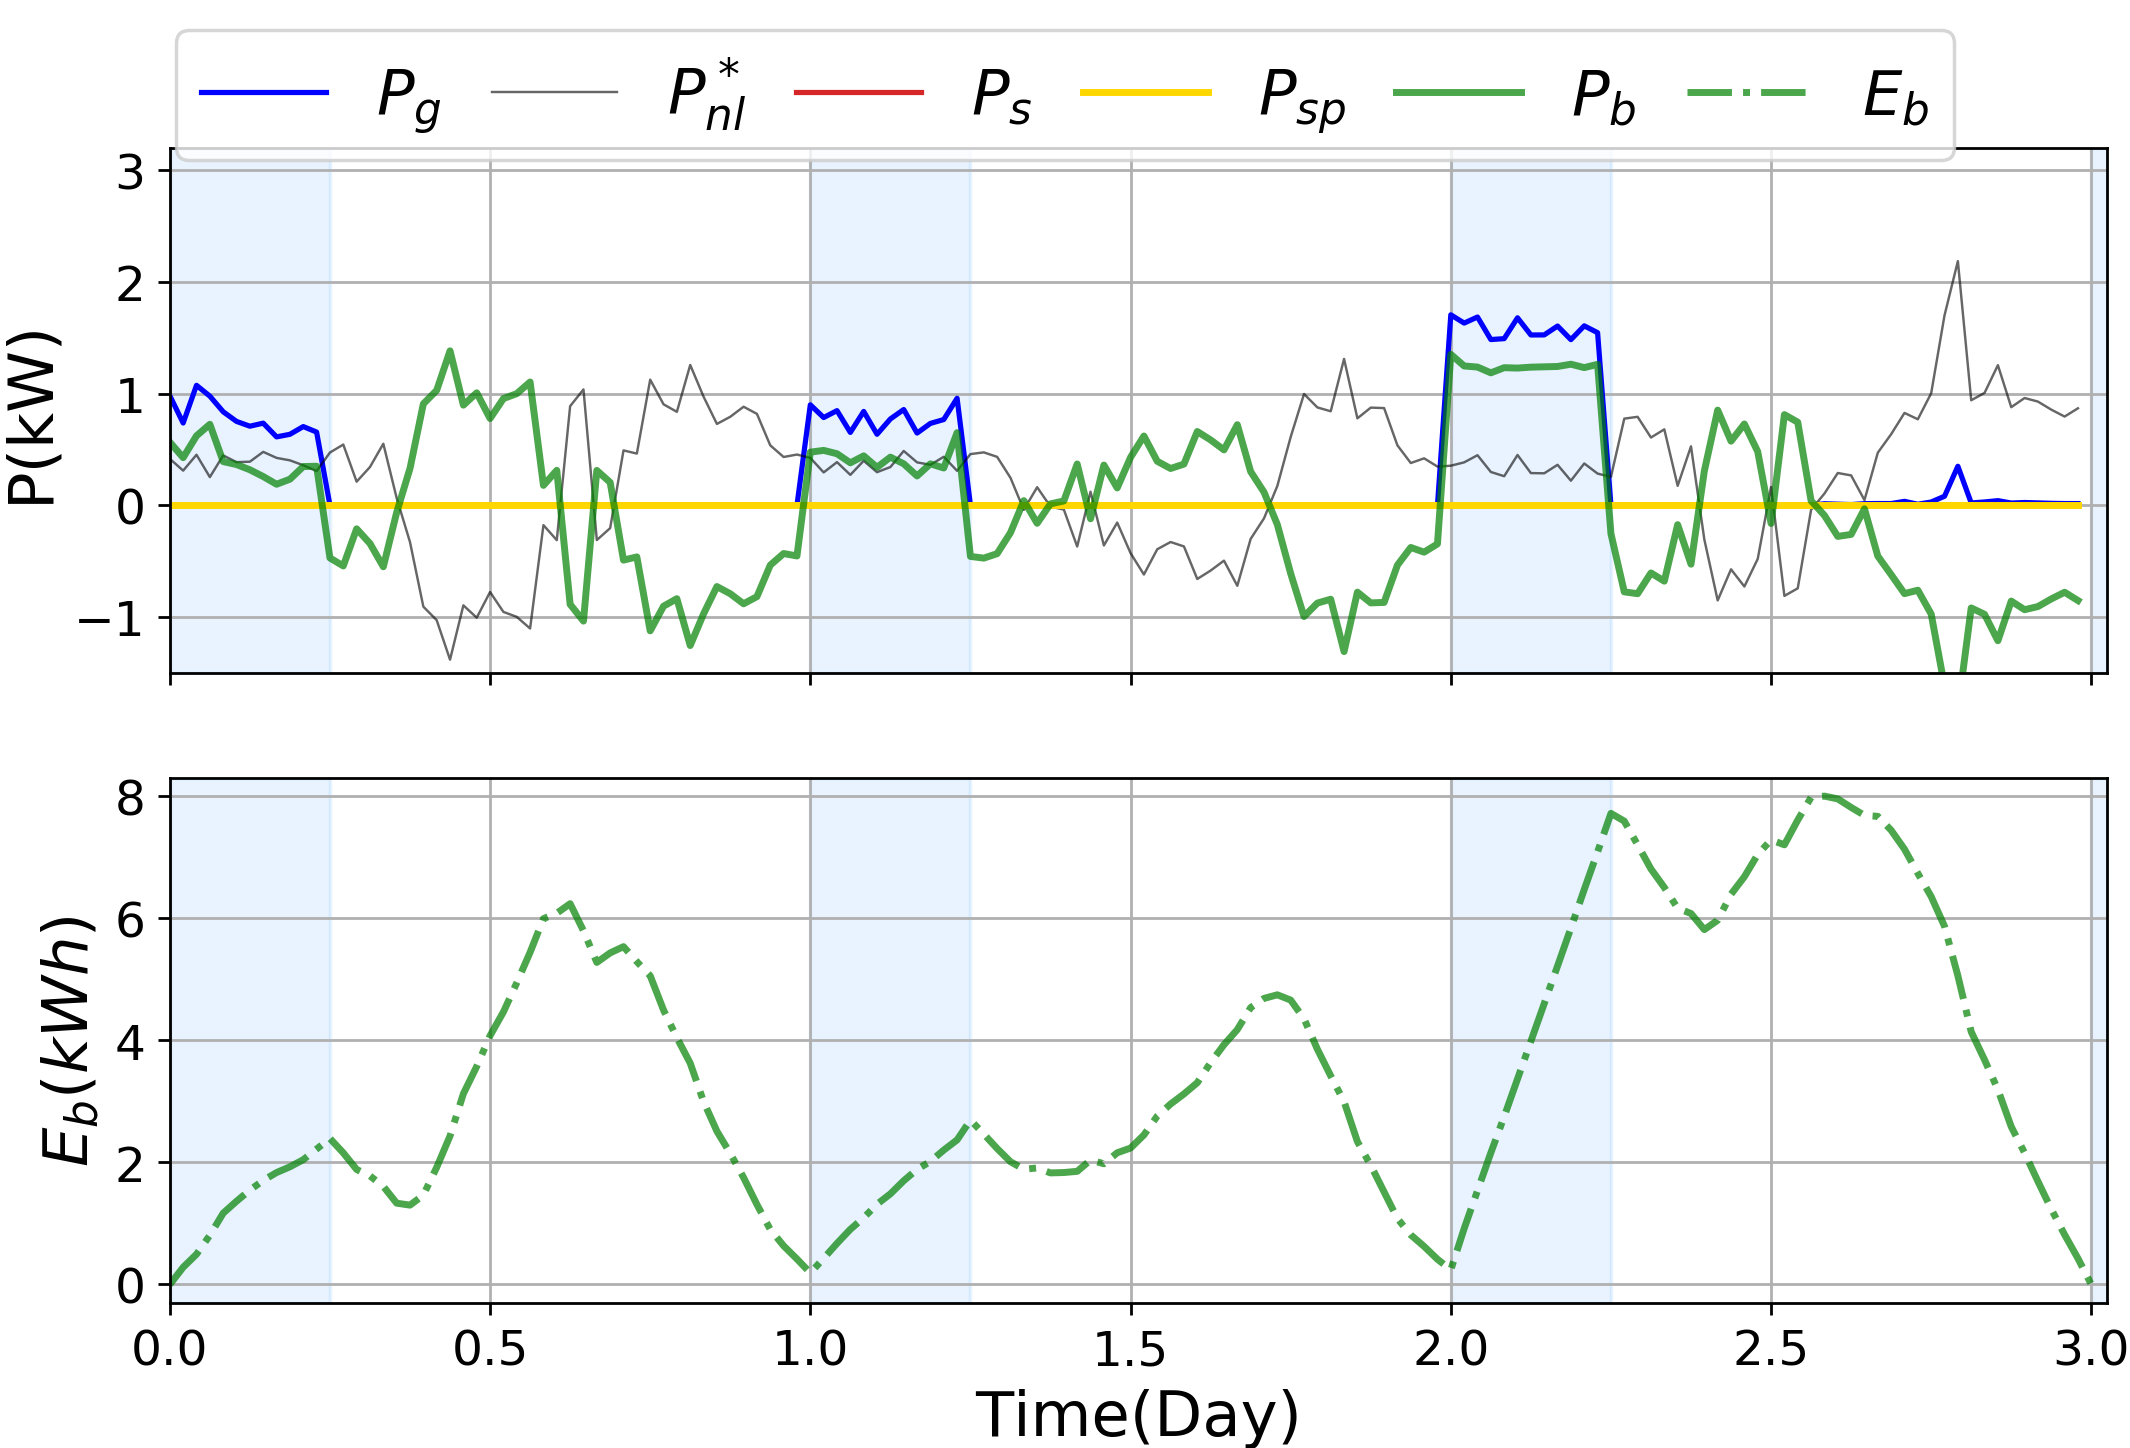
\includegraphics[height=2.5in,width=1\columnwidth]{Figures/Mc_LowFailNoOut.png}
        \caption{Low prob of failure, No outage}
        \label{fig:LOwFailNoOut}    
    \end{minipage}%
    \begin{minipage}{.01\linewidth}
      \hspace{1px}
    \end{minipage}%
    \begin{minipage}{0.49\linewidth}
        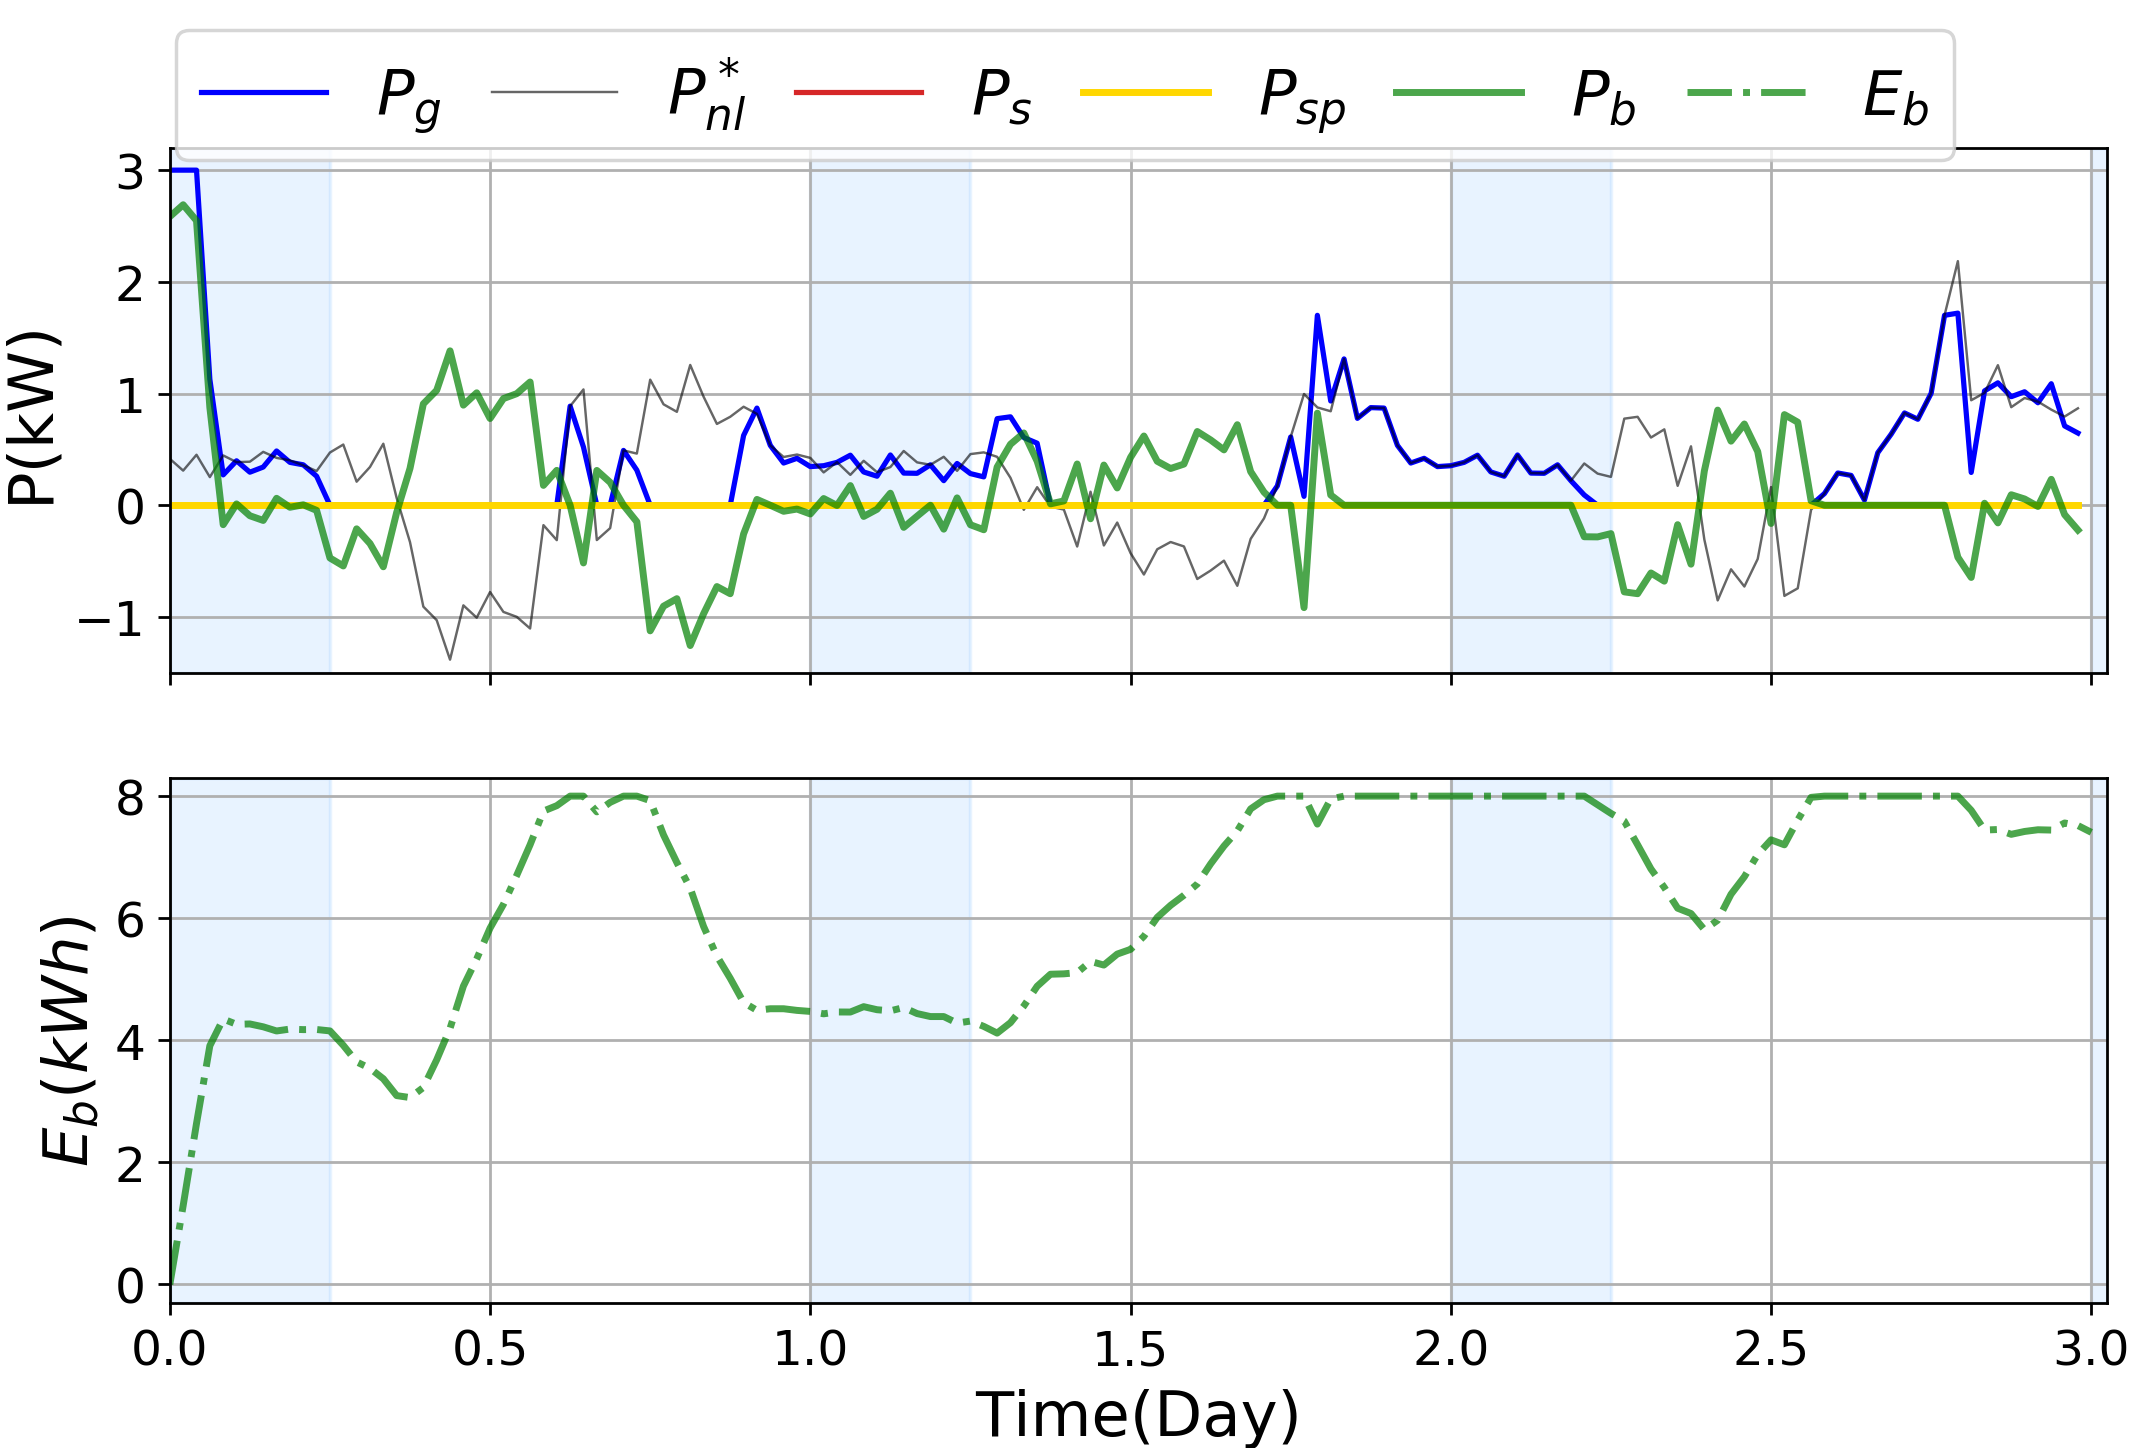
\includegraphics[height=2.5in,width=1\columnwidth]{Figures/Mc_HighFailNoOut.png}
        \caption{High prob of failure, no outage}
        \label{fig:HighFailNoOut}
    \end{minipage}
\end{figure*}

\begin{figure*}[!ht]
    \begin{minipage}{.49\linewidth}
        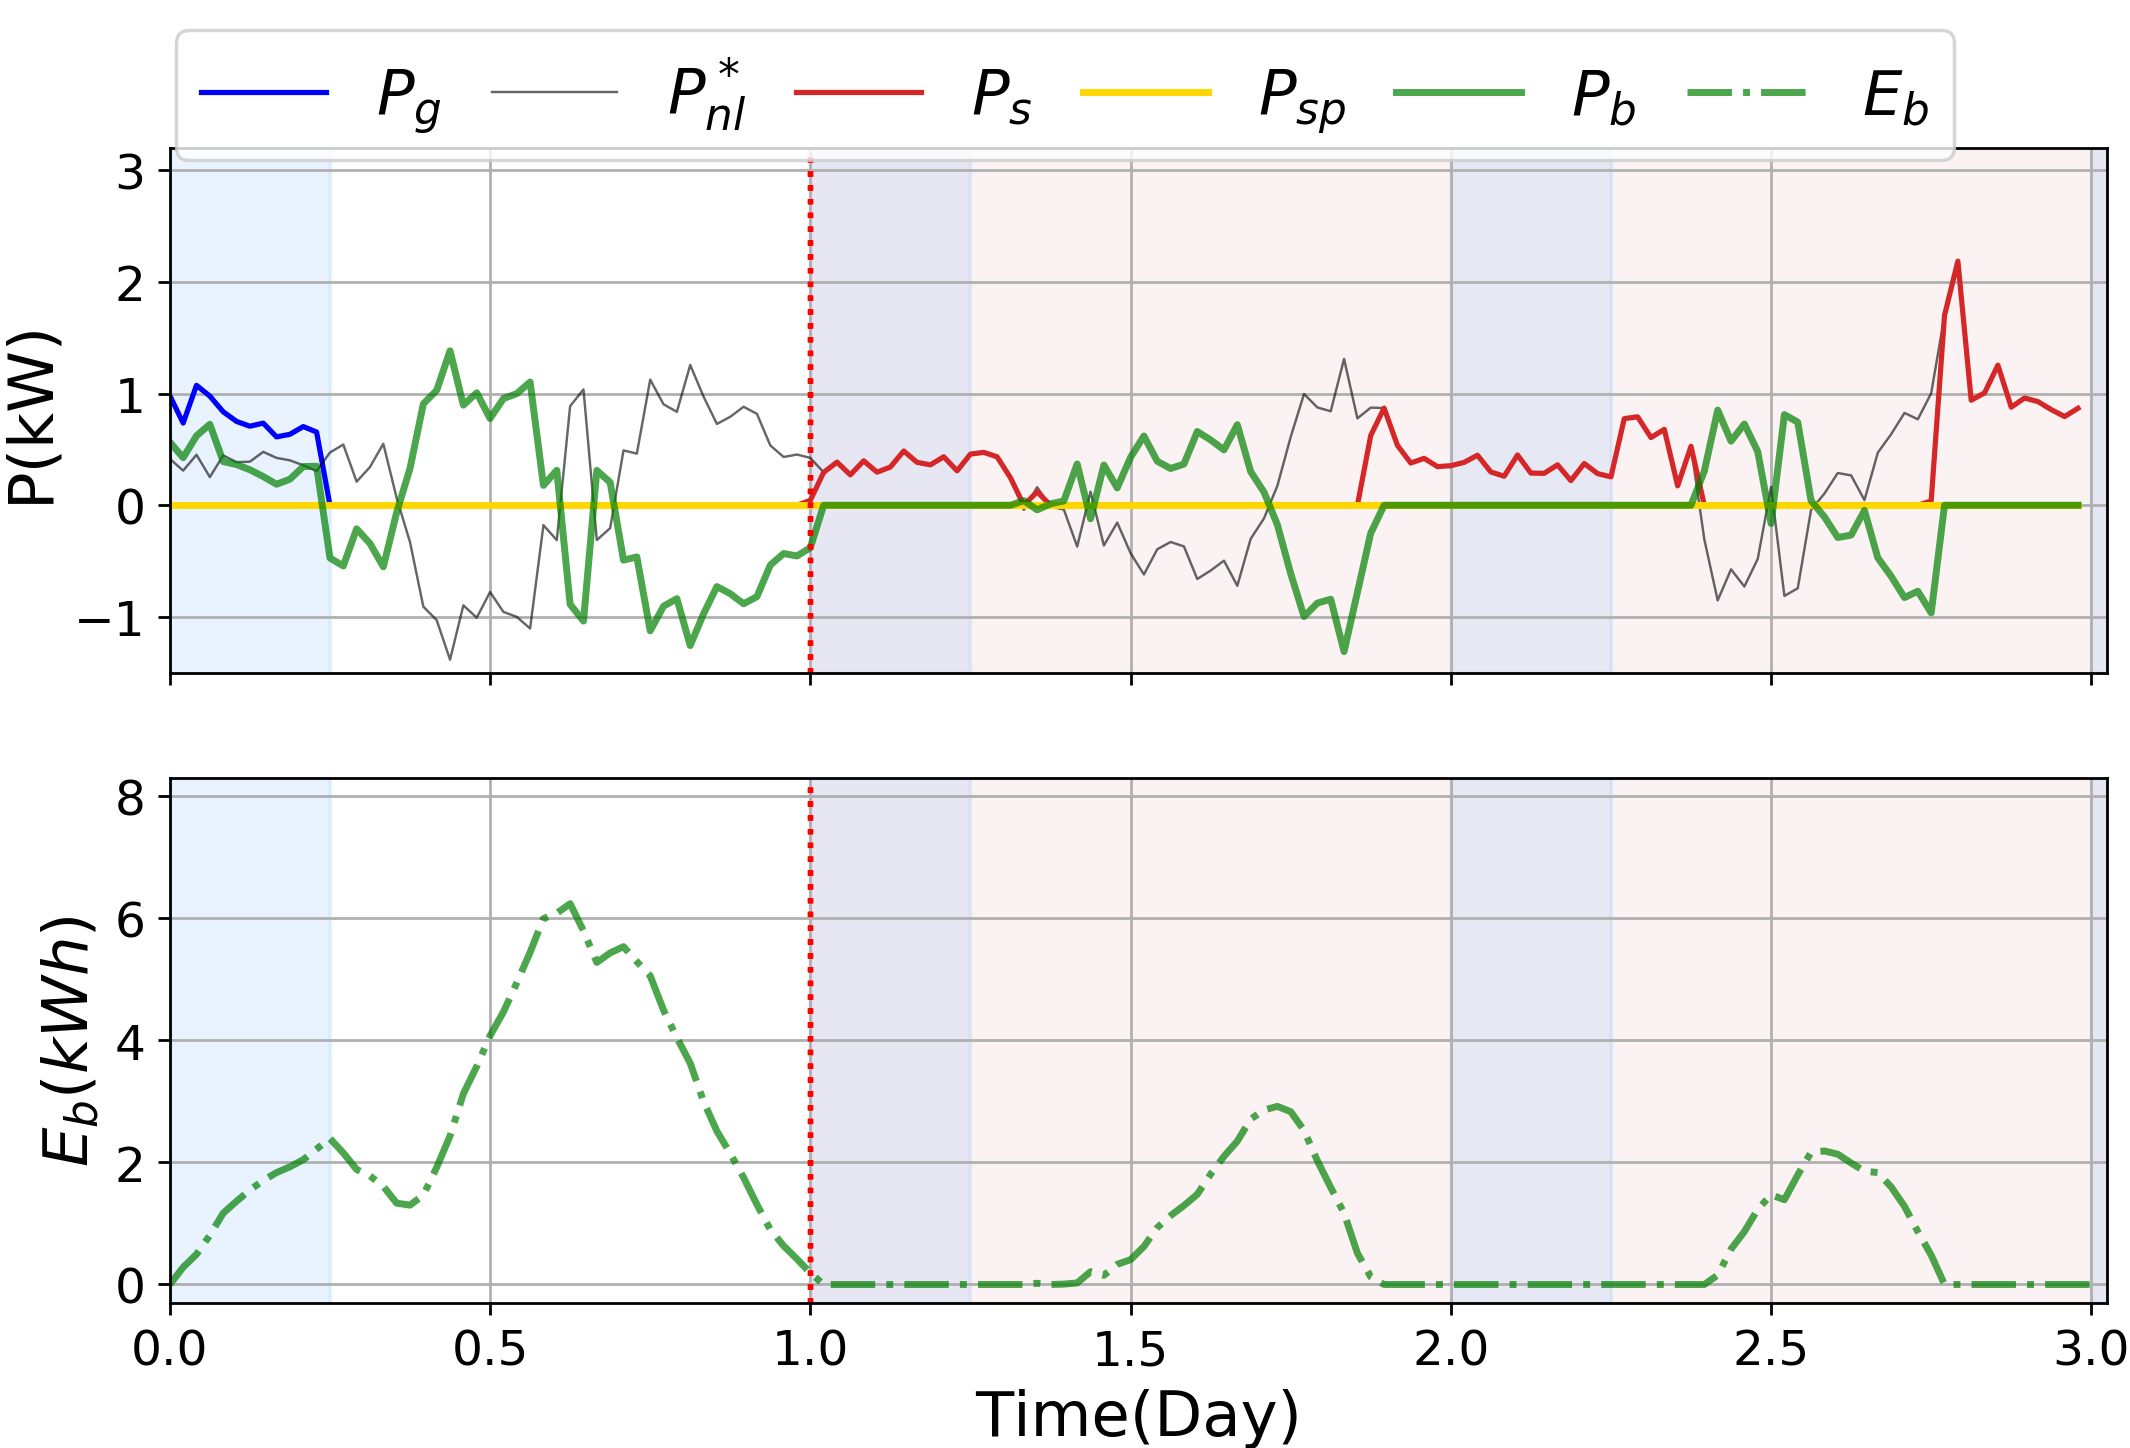
\includegraphics[height=2.5in,width=1\linewidth]{Figures/Mc_LowFailYesOut.png}
        \caption{Low prob of failure, with outage}
        \label{fig:LOwFailYesOut}    
    \end{minipage}%
    \begin{minipage}{.01\linewidth}
      \hspace{1px}
    \end{minipage}%
    \begin{minipage}{0.49\linewidth}
        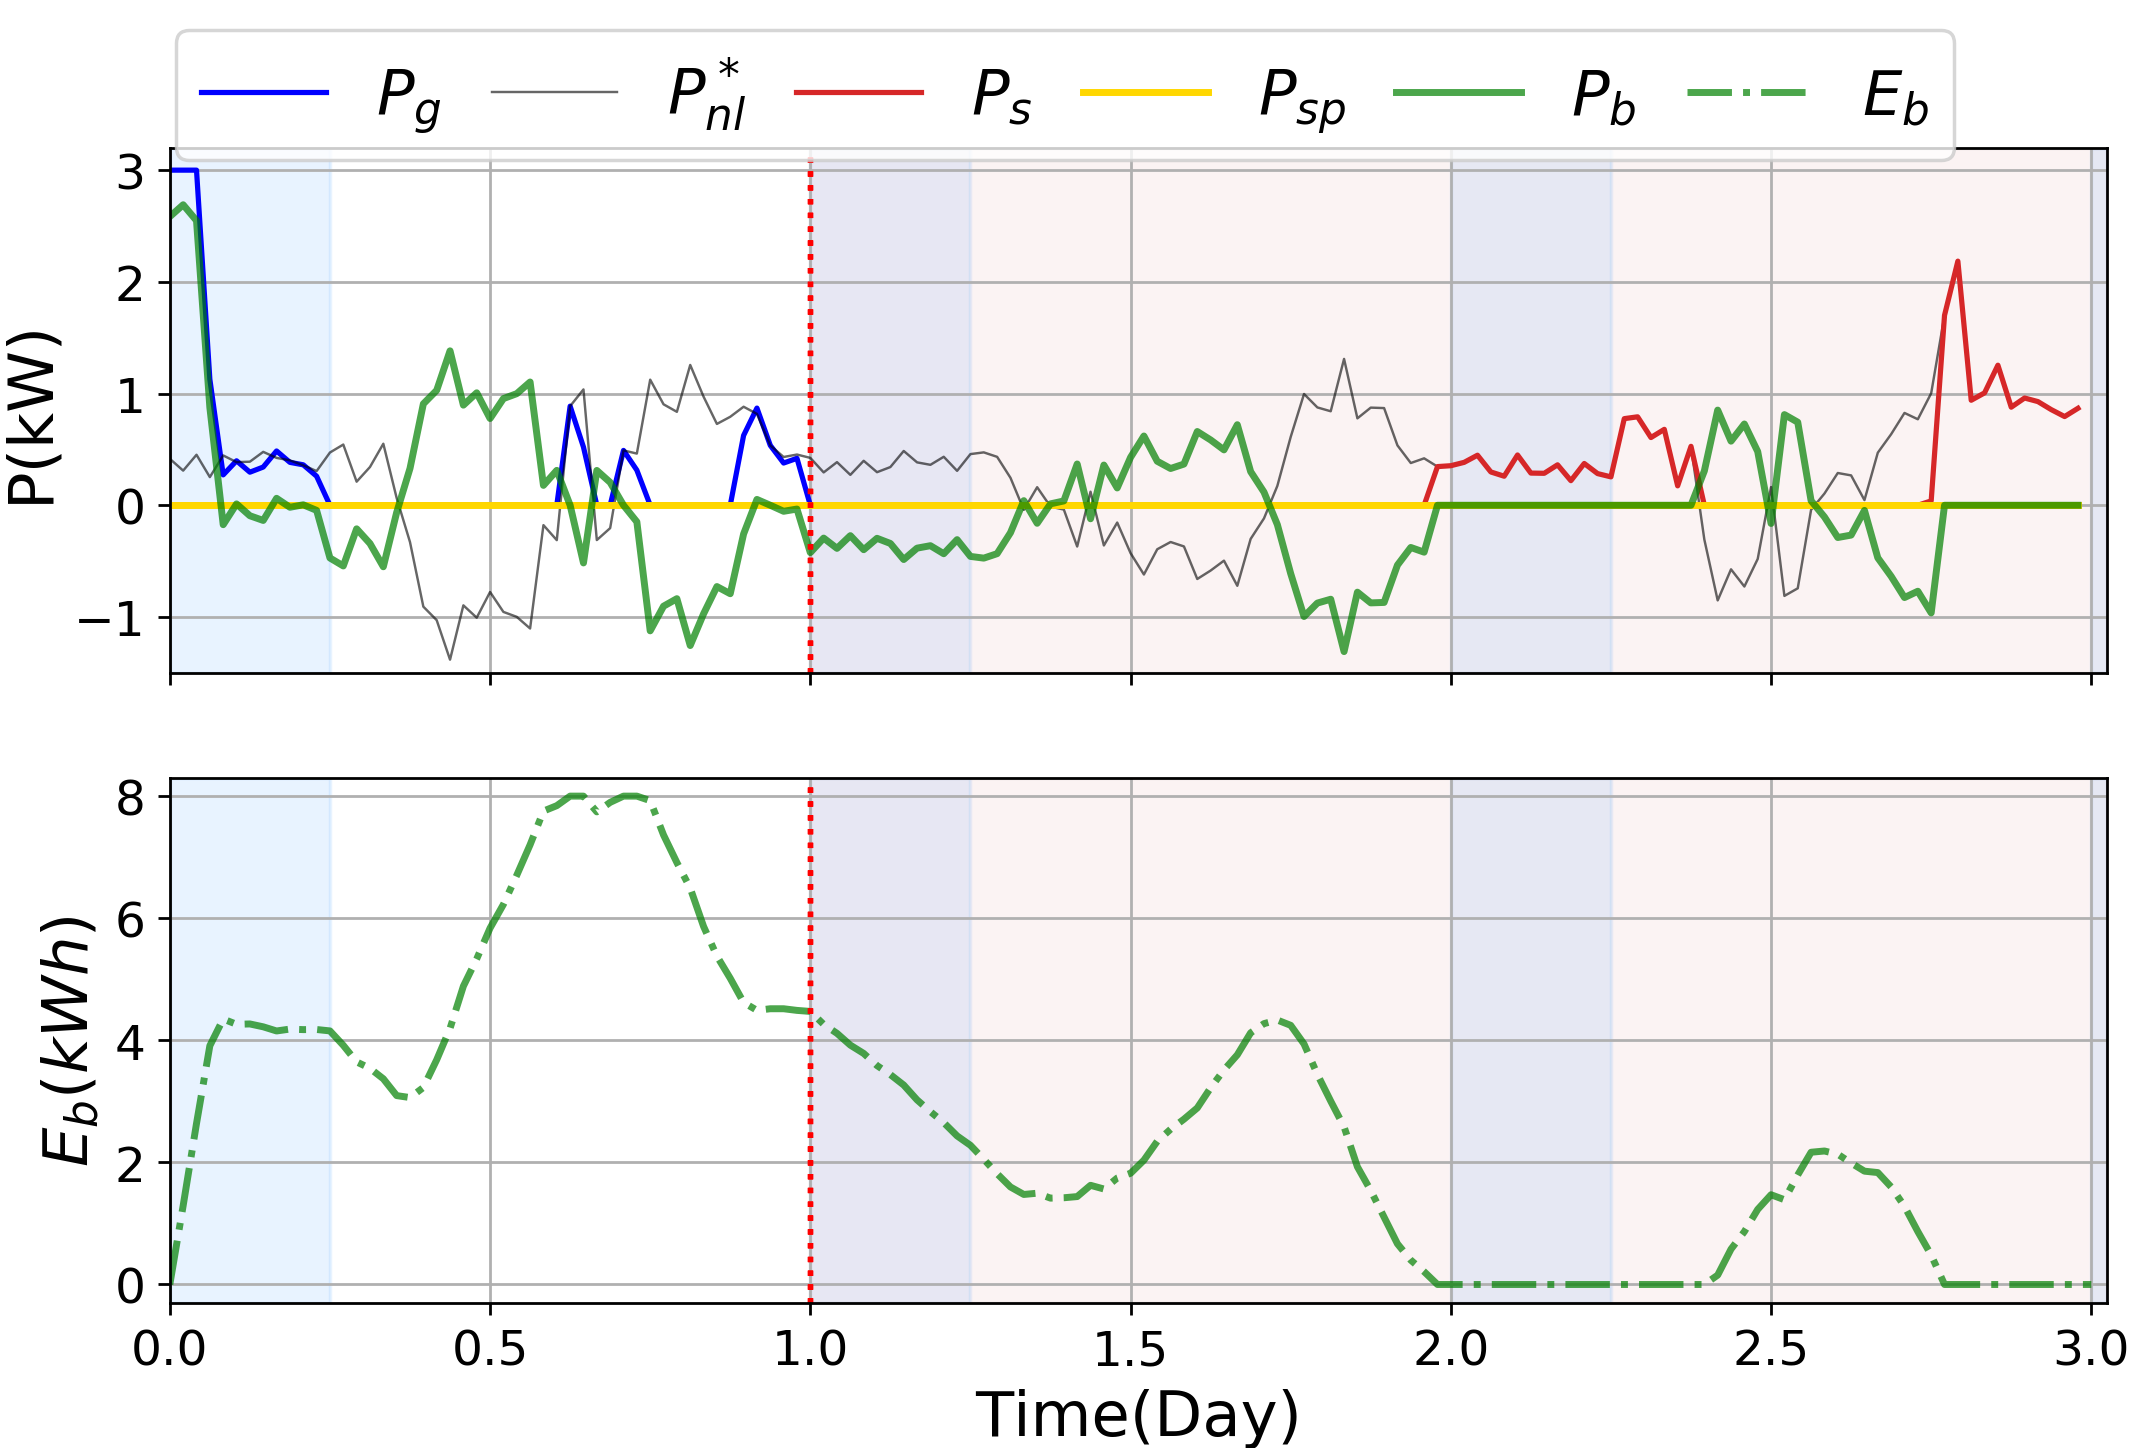
\includegraphics[height=2.5in,width=1\columnwidth]{Figures/Mc_HighFailYesOut.png} 
        \caption{High prob of failure, with outage}
        \label{fig:HighFailYesOut}
    \end{minipage}
\end{figure*}

 \begin{figure}[!htb]
        \begin{center}
                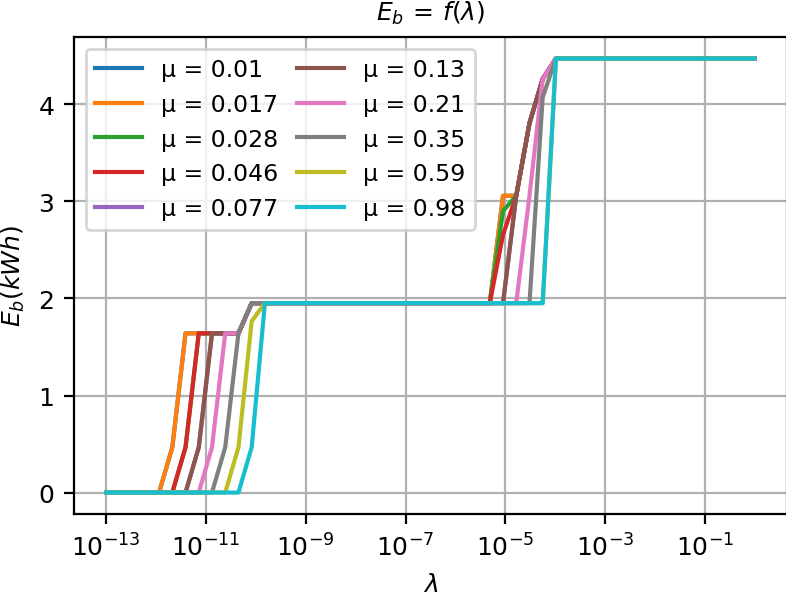
\includegraphics[width=0.9\columnwidth]{Figures/MchainMu.png}
        \end{center}
        \caption{Dynamic of the Energy inside the storage at the moment the outage occurs for the Markov chain modeling of the grid behavior for multiple repair rate.
        }
        \label{fig:MarchainVar}
\end{figure} 

 \begin{figure}[!htb]
        \begin{center}
                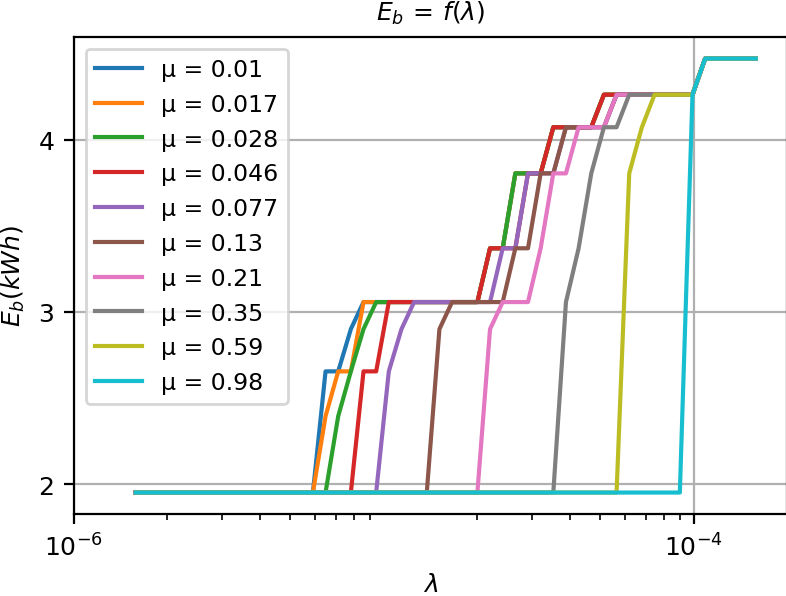
\includegraphics[width=0.9\columnwidth]{Figures/MchainMuRight.png}
        \end{center}
        \caption{Zoom on the right side of Fig. \ref{fig:MarchainVar}
        }
        \label{fig:MarchainVarRight}
\end{figure}

  For the set of simulations we have considered solely the MC's model of the grid behavior. It is the more realistic of both models since it encompass as well as the failure as the repair rate of the grid. We are mainly going to compare the behavior of the OLFC for a low and a high failure rate whether the outage actually happens or not. Fig. \ref{fig:LOwFailNoOut}, \ref{fig:HighFailNoOut} are associated with the case where the outage does not happen while Fig. \ref{fig:LOwFailYesOut}, \ref{fig:HighFailYesOut} are associated with the case where the outage does happen. The left and right figure respectively depict the behavior with a low and a high failure rate. 
  
  The higher sub-figures of each figure present the dynamic of  five electrical signal in the time. They are: the power drawn from the grid($P_g$), the energy not provided to the house ($P_s$), the wasted solar potential ($P_{sp}$), the power into the storage ($P_b$) defined all in section \ref{CaseStudy} and $P_{nl}$ which is the difference between the house demand and the solar potential i.e. $P_{nl} = P_l^* - P_{pv}^{max}$. Note that $P_{nl} < 0$ implies that there is enough solar potential to fully meet the household demand and to spare some energy into the battery. Oppositely $P_{nl} > 0$  indicates that the solar potential is not sufficient to satisfy on its own the house demand and therefore must be supplemented by the others sources. The lower sub-figures show the dynamic of the energy within the battery ($E_b$) during the simulations. Table \ref{tab:CompTable1} present the numerical result associated with Fig. \ref{fig:LOwFailNoOut}, \ref{fig:HighFailNoOut}, \ref{fig:LOwFailYesOut}, \ref{fig:HighFailYesOut}
  
  With a low failure rate, one observes that the OLFC only uses the grid during the night, especially during the off-peak hours when the electricity price is the lowest. With a high failure rate, besides on using  more of the grid during the off-peak hours (4.7kWh vs 6.5kWh) the strategy uses the grid also during the day to charge up the battery up to a certain point henceforth result in reducing the energy not provided to the house during the outage. Fig. \ref{fig:HighFailYesOut} shows that even with a high probability of failure, the OLFC from the beginning of the second day was no longer able to provided the house with its energy demand since there is no energy left inside the battery. A way to improve the strategy efficiency i.e. to reduce even more the energy not provided is to prolong the MPC horizon.
  
  Following, the next set of simulations which result are shown by Fig. \ref{fig:MarchainVar} have been done in order understand more precisely the effect of the failure rate $\lambda$ and the repair rate $\mu$ on the ROLFC. Since the quantity of energy within the battery at the instant the outage happens i.e. $E_b^{out}$ is an important factor that influences the energy not provided to the household during outages, we choose it to be the comparing factor. We have varied the repair rate $\mu$ from $0.01$ to $0.98$ with 10 data point. For each considered data point we therefore vary the failure rate $\lambda$ from a very low ($10^{-13}$) to a high ($10^{-0.01}$) probability  and recorded for each value the corresponding energy within the storage $E_b^{out}$. 
  
  Considering a constant repair rate $\lambda$, broadly one can see that the the energy within the battery increases as the the failure rate increases. To be more specific, let us divide the $\lambda$ axis in 4 intervals of interests as $[10^{-13}, 10^{-8}[$ , $[10^{-8}, 10^{-6}[$ , $[10^{-6}, 10^{-4}[$ , $[10^{-4}, 10^{-0.01}[$. At the beginning of interval 1 the failure rate is so low that the strategy does not find necessary to store some energy within the storage but, as the failure rate goes up the strategy starts storing up and stop towards the end of the current interval. The storage stays constant for the rest of the interval, as throughout the whole interval 2 until the beginning of interval 3. In the latter the strategy resumes increasing the stored energy as the failure rate increases but eventually stopped and stay constant for the remaining part of interval 3 and 4 no matter how high the failure rate gets. 
  
  Figure \ref{fig:MarchainVarRight} is a zoom on the interval 3 of Fig. \ref{fig:MarchainVar}. One can conclude from it that for a constant failure rate, the lower the repair rate, the higher is the energy within the storage when the outage happens. This goes with the logical intuition which is the more time the system will undergo a default period, the more important should be the energy within the storage when the default appears in order to reduce the user discomfort during the outage period. 
 
\section{Conclusion}\label{conclusion}
In this paper we have developed the ROLFC for EMS in order to integrate a probabilistic model of grid outages. The stochastic consideration is rewritten into a deterministic optimization using an auxiliary variable. This technique has been used in a study case with two different grids outages models. This showed the impact of the outage  failure rate on the behavior of the MPC.

 Our next step is to investigate how to improve even more the resiliency of the controller during an outage. The improved controller, during outages should be able to actively reduce or not the load demand both according to the user will and the grid repair rate. We are also planing on considering a more realistic model of the load demand and the sun potential which in that case will be considered to be stochastic.
 

\begin{thebibliography}{00}


\bibitem{OnlnCER} CEER(Council of European Energy Regulators),``Ref. C14-EQS-62-03'', Benchmarking Report 5.2 on the Continuity of Electricity Supply,Online at http://www.ceer.eu/,accessed 06-September-2018.

\bibitem{HGhRBo2015} Hamed Ghasemieh, Boudewijn R. Haverkort, Marijn R. Jongerden and Anne Remke, ``Energy Resilience Modeling for Smart Houses'', Proceedings of the 45th Annual IEEE/IFIP International Conference on Dependable Systems and Networks, 2015, vol. 45, pp.275--286.

\bibitem{RRoFBe2014} R. Roche, F. Berthold, F. Gao, F. Wang, A. Ravey and S. Williamson, "A model and strategy to improve smart home energy resilience during outages using vehicle-to-home", IEEE International Electric Vehicle Conference (IEVC), Florence, 2014, pp. 1-6.

\bibitem{JMaHJa2016} Marijn R. Jongerden, Jannik Hüls, Anne Remke and Boudewijn R. Haverkort, ``Does Your Domestic Photovoltaic Energy System Survive Grid Outages ?'', Energies, 2016, vol. 9.

\bibitem{JPrPHa2019} Jesse-James Prince A., Pierre Haessig, Romain Bourdais and Herve Gueguen, ``Resilience in energy management system: A study case'', IFAC-PapersOnLine, 2019, Vol. 52, Issue 4, pp. 395--400.

\bibitem{Deb2014} Deb Kalyanmoy, ``Multi-objective Optimization'', in Search Methodologies: Introductory Tutorials in Optimization and Decision Support Techniques, 2014, pp. 403--449.

\bibitem{ECaCbo2007} Eduardo F. Camacho and Carlos Bordons Alba, ``Model Predictive Control'', in Advanced Textbooks in Control and Signal Processing, 2nd ed., 2017.

\bibitem{BenTal2009} A. Ben-Tal, L. El Ghaoui  and A. Nemirovski, ``Robust Optimization'', 2009.

\bibitem{Ankopa1995} Andr\'as Pr\'ekopa, ``Stochastic Programming'', 1995.

\bibitem{AChWCo1958} A. Charnes, W. W. Cooper, G. H. Symond, ``Cost Horizons and Certainty Equivalents: An Approach to Stochastic Programming of Heating Oil'', Management Science, 1958, vol. 4, pp.235--263.

\bibitem{AChWCo1959} A. Charnes and W. W. Cooper, ``Chance-Constrained Programming'', Management Science, 1959, vol. 6, pp.73--79.


\bibitem{SLuAJo2014} Sergio Lucia, Joel A.E. Andersson, Heiko Brandt, Moritz Diehl and Sebastian Engell, ``Handling uncertainty in economic nonlinear model predictive control: A comparative case study'', Journal of Process Control, 2014, vol. 24, pp.1247--1259.

\bibitem{YBarRSi1969} Y. {Bar-Shalom} and R. {Sivan}, ``On the optimal control of discrete-time linear systems with random parameters'', IEEE Transactions on Automatic Control, 1969, vol. 14, pp.3--8.

\bibitem{RBiRna1992} Roy Billinton and Ronald N. Allan, ``Reliability Evaluation of Engineering Systems, 1992,.

\end{thebibliography}

\end{document}


